\begin{figure}[ht]
    \centering
    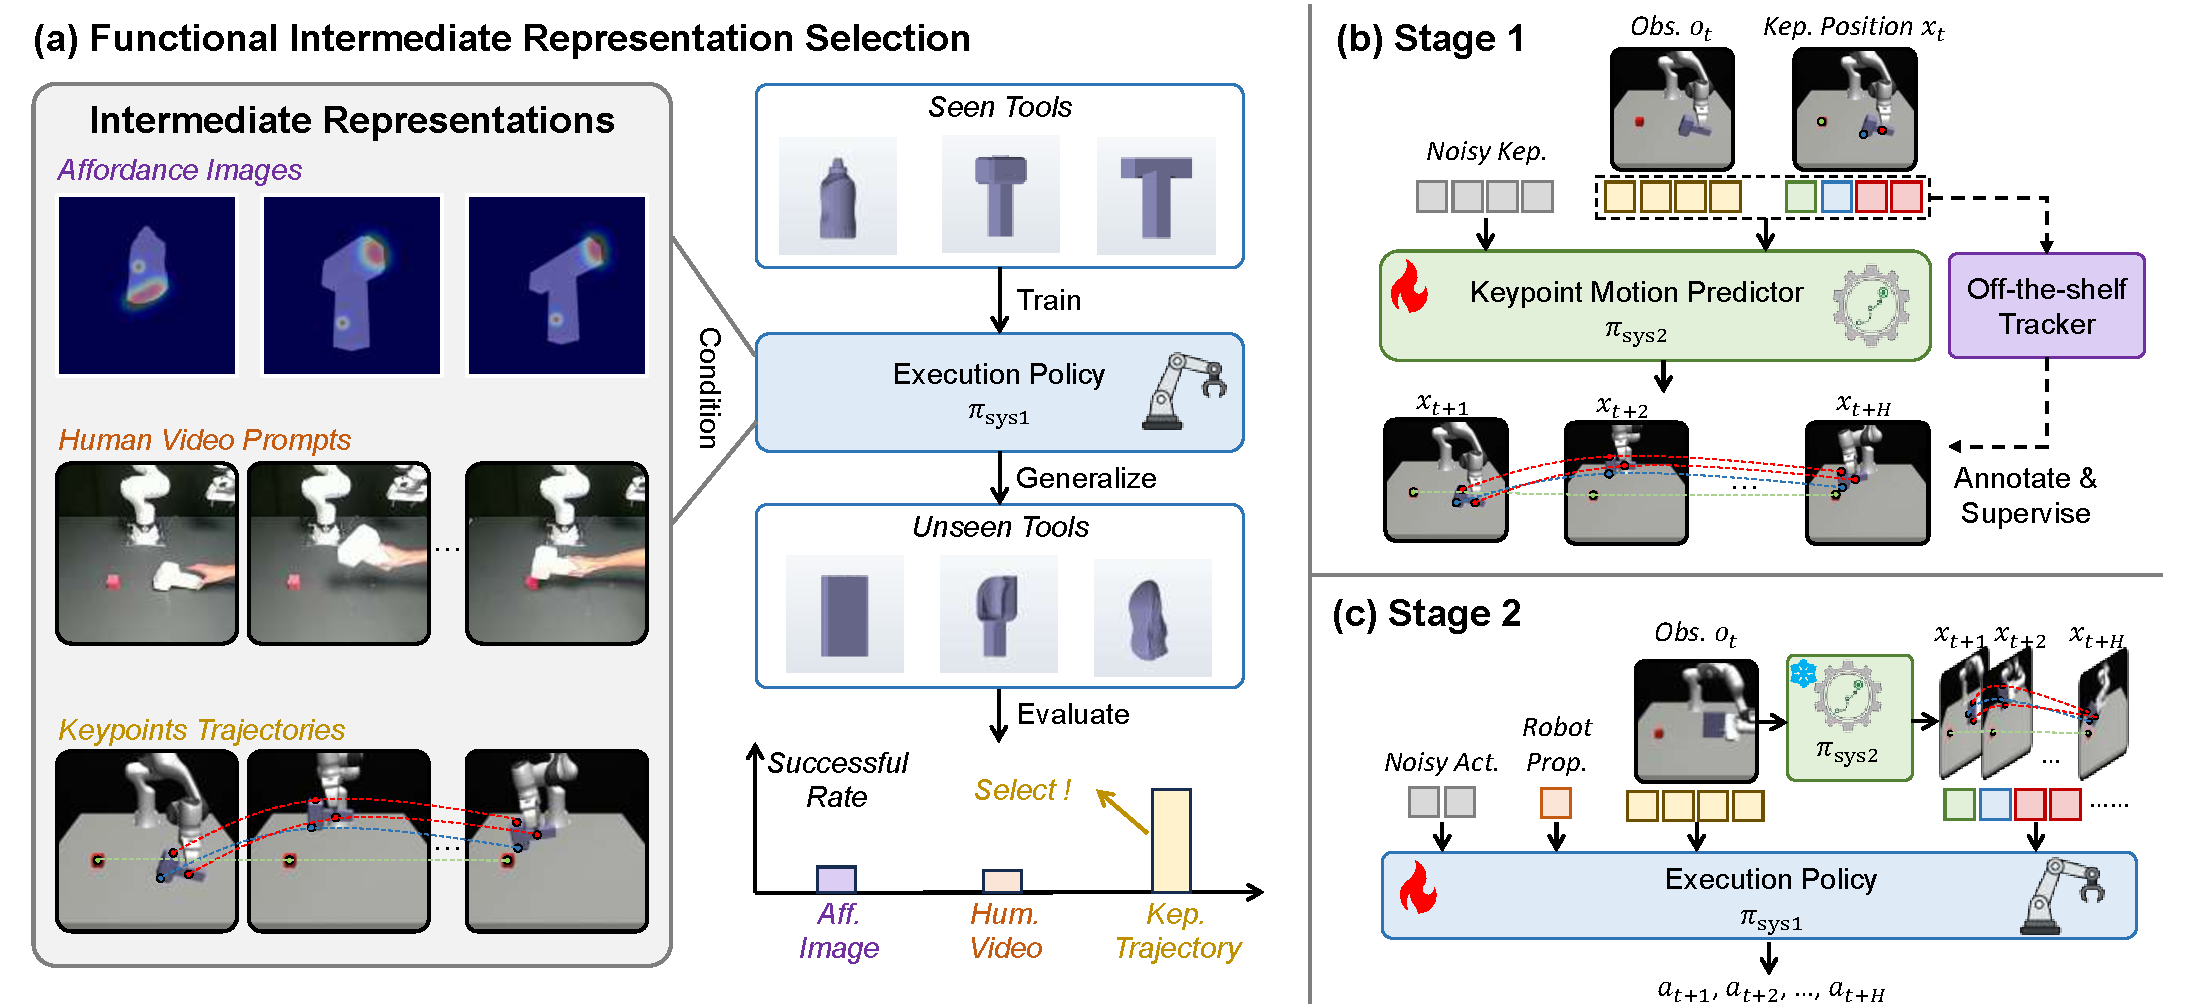
\includegraphics[width=1.0\linewidth]{figures/main_pipeline.pdf}
    \caption{
    \textbf{Overview of the \algoname{}.} (a) Evaluation and selection of functional intermediate representations. (b) In Stage 1, the System-2 planner learns to predict future keypoint-based functional plans from action-free observations. (c) In Stage 2, the System-1 execution policy grounds the predicted functional plans into executable robot actions.
    }
    \label{fig:functional_generalization_pipeline}
\end{figure}

\section{Methods}
\label{sec:method}

% \subsection{Problem Formulation}
% Our Generalizable Function Plan and Execution (\algoname{}) policy follows a human-inspired dual-system architecture. Given the visual observation $o_{t}$ at time step $t$, the System-2 policy $\pi_{\mathrm{sys}\text{-}2}$ predicts a high-level functional plan, denoted as $x_{t:t+H} = \pi_{\mathrm{sys}2}(o_{t})$, where $x_{t:t+H}$ serves as a trade-off representation over a future horizon $H$. This representation is more structured than dense visual features and more abstract than low-level motor commands, making it suitable for bridging functional planning and action grounding. The System-1 policy $\pi_{\mathrm{sys}1}$ then grounds this plan into executable actions, denoted as ${a}_{t:t+H} = \pi_{\mathrm{sys}\text{-}1}(o_{t}, q_{t}, {x}_{t:t+H})$, by conditioning on the visual observation ${o}_{t}$, the robot proprioceptive state $q_{t}$, and the predicted trade-off representation $x_{t:t+H}$.

% To achieve this goal, we assume access to two types of training data. The first is a large-scale action-free dataset $\mathcal{D}_{U} = \{(o^{i}_{t}, x^{i}_{t:t+H})\}_{i=1}^{N_{U}}$, where each sample contains a visual observation and its corresponding trade-off representation, without requiring robot action labels. The second is a smaller action-labeled dataset $\mathcal{D}_{L} = \{(o^{i}_{t}, q^{i}_{t}, a^{i}_{t:t+H})\}_{i=1}^{N_{L}}$, where each sample provides the visual observation, robot proprioceptive state, and action trajectory label. We first pretrain the System-2 policy $\pi_{\mathrm{sys}\text{-}2}$ on $\mathcal{D}_{U}$ to learn function-relevant planning from action-free data. We then integrate the pretrained System-2 module with the System-1 execution policy and finetune the overall \algoname{} policy on $\mathcal{D}_{L}$, enabling the model to translate high-level functional plans into executable robot actions.

% Our Generalizable Function Plan and Execution (\algoname{}) policy follows a human-inspired dual-system architecture. Assume that two datasets are accessible: a large-scale action-free dataset $\mathcal{D}_{U}=\{(\mathbf{O}^{(i)}, \mathbf{X}^{(i)})\}_{i=1}^{N_U}$, where each sample contains a sequence of visual observations $\mathbf{O}^{(i)}=\{o_{t}^{(i)}\}_{t=1}^{T}$ and the corresponding trade-off representations $\mathbf{X}^{(i)}=\{x_{t}^{(i)}\}_{t=1}^{T}$; and a smaller action-labeled robotic dataset $\mathcal{D}_{L}=\{(\mathbf{O}^{(i)}, \mathbf{Q}^{(i)}, \mathbf{A}^{(i)})\}_{i=1}^{N_L}$, where $\mathbf{Q}^{(i)}=\{q_{t}^{(i)}\}_{t=1}^{T}$ denotes the robot proprioceptive states and $\mathbf{A}^{(i)}=\{a_{t}^{(i)}\}_{t=1}^{T}$ denotes the action labels. Our objective is to first learn a System-2 policy $\pi_{\mathrm{sys}2}$ from $\mathcal{D}_{U}$, which predicts a future function-relevant plan from the current visual observation and trade-off representation: $x_{t:t+H}=\pi_{\mathrm{sys}2}(o_t,x_t)$. We then finetune both $\pi_{\mathrm{sys}2}$ and the System-1 policy $\pi_{\mathrm{sys}1}$ on $\mathcal{D}_{L}$, so that the predicted functional plan can be grounded into executable actions: $a_{t:t+H}=\pi_{\mathrm{sys}1}(o_t,q_t,\pi_{\mathrm{sys}2}(o_t,x_t))$. At test time, for an unseen tool-use sample $(\mathbf{O}^{*}, \mathbf{Q}^{*}, \mathbf{A}^{*}) \notin \mathcal{D}_{L}$, \algoname{} generates the action trajectory $a_{t:t+H}^{*}=\pi_{\mathrm{sys}1}(o_t^{*},q_t^{*},\pi_{\mathrm{sys}2}(o_t^{*},x_t^{*}))$ to accomplish the hitting function.

% Our Generalizable Function Plan and Execution (\algoname{}) policy follows a human-inspired dual-system architecture. Assume that two datasets are accessible: a large-scale action-free dataset $\mathcal{D}_{U}=\{(\mathbf{O}^{(i)}, \mathbf{X}^{(i)})\}_{i=1}^{N_U}$, where each sample contains a sequence of visual observations $\mathbf{O}^{(i)}=\{o_{t}^{(i)}\}_{t=1}^{T}$ and the corresponding trade-off representations $\mathbf{X}^{(i)}=\{x_{t}^{(i)}\}_{t=1}^{T}$; and a smaller action-labeled robotic dataset $\mathcal{D}_{L}=\{(\mathbf{O}^{(i)}, \mathbf{X}^{(i)}, \mathbf{Q}^{(i)}, \mathbf{A}^{(i)})\}_{i=1}^{N_L}$, where $\mathbf{Q}^{(i)}=\{q_{t}^{(i)}\}_{t=1}^{T}$ denotes the robot proprioceptive states and $\mathbf{A}^{(i)}=\{a_{t}^{(i)}\}_{t=1}^{T}$ denotes the action labels. Our objective is to learn a System-2 policy $\pi_{\mathrm{sys}2}$ from $\mathcal{D}_{U}$, which predicts a future function-relevant plan from the current visual observation and trade-off representation: $x_{t:t+H}=\pi_{\mathrm{sys}2}(o_t,x_t)$. We then finetune both $\pi_{\mathrm{sys}2}$ and the System-1 policy $\pi_{\mathrm{sys}1}$ on $\mathcal{D}_{L}$, so that the predicted functional plan can be grounded into executable actions: $a_{t:t+H}=\pi_{\mathrm{sys}1}(o_t,q_t,\pi_{\mathrm{sys}2}(o_t,x_t))$. At test time, for an unseen tool-use sample $(\mathbf{O}^{*}, \mathbf{Q}^{*}, \mathbf{A}^{*}) \notin \mathcal{D}_{L}$, \algoname{} policy is expected to generate the action trajectory $a_{t:t+H}^{*}=\pi_{\mathrm{sys}1}(o_t^{*},q_t^{*},\pi_{\mathrm{sys}2}(o_t^{*},x_t^{*}))$ to accomplish the hitting function.

% \subsection{Problem Formulation}
% Our Generalizable Functional Plan and Execution (\algoname{}) policy follows a human-inspired dual-system architecture, where a high-level System-2 planner predicts function-relevant future states and a low-level System-1 policy grounds them into executable robot actions. 
% We assume that two types of datasets are accessible. 
% The first is a large-scale action-free dataset 
% $\mathcal{D}_{U}=\{(\mathbf{O}^{(i)}, \mathbf{X}^{(i)})\}_{i=1}^{N_U}$, 
% where $\mathbf{O}^{(i)}=\{o_t^{(i)}\}_{t=1}^{T}$ denotes a sequence of visual observations, and 
% $\mathbf{X}^{(i)}=\{x_t^{(i)}\}_{t=1}^{T}$ denotes the corresponding functional intermediate representations which describe functional-relevant future states. 
% % These representations describe task-relevant functional states, such as future keypoint trajectories, without requiring robot action labels. 
% The second is a smaller action-labeled robotic dataset 
% $\mathcal{D}_{L}=\{(\mathbf{O}^{(i)}, \mathbf{X}^{(i)}, \mathbf{Q}^{(i)}, \mathbf{A}^{(i)})\}_{i=1}^{N_L}$, 
% where $\mathbf{Q}^{(i)}=\{q_t^{(i)}\}_{t=1}^{T}$ means robot proprioceptive states and 
% $\mathbf{A}^{(i)}=\{a_t^{(i)}\}_{t=1}^{T}$ represents ground-truth actions.

% Given observation $o_t$ and functional representation $x_t$ at time-step $t$, the System-2 planner 
% $\pi_{\mathrm{sys2}}$ predicts a future functional plan over horizon $H$:
% \begin{equation}
%     \hat{\mathbf{X}}_{t:t+H}
%     =
%     \pi_{\mathrm{sys2}}(o_t, x_t).
% \end{equation}
% The System-1 execution policy $\pi_{\mathrm{sys1}}$ then grounds this predicted plan into an action trajectory conditioned on the current observation and robot state:
% \begin{equation}
%     \hat{\mathbf{A}}_{t:t+H}
%     =
%     \pi_{\mathrm{sys1}}(o_t, q_t, \hat{\mathbf{X}}_{t:t+H}).
% \end{equation}
% % Therefore, \algoname{} first learns functional planning from action-free data and then learns action grounding from limited action-labeled demonstrations. 
% % At test time, given an unseen tool, \algoname{} predicts a future functional plan and grounds it into robot actions to accomplish the same hitting function with the novel tool.
% Consequently, the objective of \algoname{} is to learn a functional planner from action-free data and an execution policy from limited action-labeled data, such that the predicted functional plans can be grounded into executable robot actions. 
% At test time, given an unseen tool, the \algoname{} policy predicts a future functional plan and translates it into actions to accomplish the same hitting function with the novel tool.






\subsection{Problem Formulation}
% Our Functional Reasoning and Grounded Execution (\algoname{}) policy follows a dual-system architecture for functional generalization in tool-use manipulation. \lw{introduce the problem first, something like MDP}
% Given a task function, such as hitting a target object, the goal is to learn a policy that can accomplish the same function with novel tools whose visual appearances and geometries differ from those observed during training.

% We assume that two types of datasets are available. 
% The first is a large-scale action-free dataset 
% $\mathcal{D}_{U}=\{(\mathbf{O}^{(i)}, \mathbf{X}^{(i)})\}_{i=1}^{N_U}$, 
% where $\mathbf{O}^{(i)}=\{\mathbf{o}^{(i)}_t\}_{t=1}^{T}$ denotes a sequence of visual observations, and 
% $\mathbf{X}^{(i)}=\{\mathbf{x}^{(i)}_t\}_{t=1}^{T}$ denotes the corresponding functional intermediate representations that describe function-relevant future states. 
% The second is a smaller action-labeled robotic dataset 
% $\mathcal{D}_{L}=\{(\mathbf{O}^{(i)}, \mathbf{X}^{(i)}, \mathbf{Q}^{(i)}, \mathbf{A}^{(i)})\}_{i=1}^{N_L}$, 
% where $\mathbf{Q}^{(i)}=\{\mathbf{q}^{(i)}_t\}_{t=1}^{T}$ represents robot proprioceptive states and 
% $\mathbf{A}^{(i)}=\{\mathbf{a}^{(i)}_t\}_{t=1}^{T}$ denotes ground-truth robot actions.

% The objective of \algoname{} is decoupled into two sub-problems.
% First, a System-2 planner learns from action-free data to predict a functional plan in the space of intermediate representations. 
% Second, a System-1 execution policy grounds the predicted functional plan into executable robot actions via finetuning on action-labeled data. 
% This decomposition allows \algoname{} to leverage scalable action-free data for functional reasoning, while using limited robotic demonstrations for action grounding.

% \lw{
% We formulate functional generalization in tool-use manipulation as a Markov Decision Process (MDP), where the state $\mathbf{s}_t$ consists of the visual observation $\mathbf{o}_t$ and the robot proprioceptive state $\mathbf{q}_t$, and the action $\mathbf{a}_t$ is a motor command. A task function (e.g., hitting a target) is associated with a set of seen tools $\mathcal{T}_{\text{seen}}$ used for training and a disjoint set of unseen tools $\mathcal{T}_{\text{unseen}}$ used for evaluation, where the function stays fixed but the tool, its appearance, and its required motion all change. Two types of data are available for learning. The first is a large-scale action-free dataset $\mathcal{D}_{U}=\{(\mathbf{O}^{(i)}, \mathbf{X}^{(i)})\}_{i=1}^{N_U}$, consisting of visual observations $\mathbf{O}^{(i)}=\{\mathbf{o}^{(i)}_t\}_{t=1}^{T}$ and corresponding functional intermediate representations $\mathbf{X}^{(i)}=\{\mathbf{x}^{(i)}_t\}_{t=1}^{T}$ (e.g., 2D keypoint trajectories from an off-the-shelf tracker), which is abundant since it requires no robot labels. The second is a smaller action-labeled robotic dataset $\mathcal{D}_{L}=\{(\mathbf{O}^{(i)}, \mathbf{X}^{(i)}, \mathbf{Q}^{(i)}, \mathbf{A}^{(i)})\}_{i=1}^{N_L}$, which additionally provides proprioceptive states $\mathbf{Q}^{(i)}$ and ground-truth actions $\mathbf{A}^{(i)}$ but is costly to collect, so $|\mathcal{D}_L| \ll |\mathcal{D}_U|$. This data asymmetry, together with the affordance-to-action gap discussed in Sec.~\ref{sec:intro}, motivates a two-stage decomposition: \algoname{} learns a future-state predictor on $\mathcal{D}_U$ that forecasts the functional intermediate representation from observations, and an execution policy on $\mathcal{D}_L$ that grounds the predicted representation into robot actions.
% }

We formulate functional generalization in tool-use manipulation as a Markov Decision Process (MDP), where the state $\mathbf{s}_t$ consists of the visual observation $\mathbf{o}_t$, the proprioceptive state $\mathbf{q}_t$, and optionally a functional intermediate representation $\mathbf{x}_t$ (e.g., affordance images, human video prompts, or keypoint trajectories) that carries function-relevant cues bridging perception and action, and the action $\mathbf{a}_t$ is the motor command. A task function (e.g., hitting a target) is defined over seen tools $\mathcal{T}_{\text{seen}}$ for training and disjoint unseen tools $\mathcal{T}_{\text{unseen}}$ for evaluation, where the function stays fixed but the tool, its appearance, and the required contact positions and motions all change.


%We formulate functional generalization in tool-use manipulation as a Markov Decision Process (MDP), where the state $\mathbf{s}_t$ consists of the visual observation $\mathbf{o}_t$, the robot proprioceptive state $\mathbf{q}_t$, and optionally a functional intermediate representation $\mathbf{x}_t$, while action $\mathbf{a}_t$ denotes the motor command.
%The functional intermediate representation is expected to carry function-relevant cues that bridge perception and action, such as contact regions, target locations, or motion patterns. It can be instantiated in various forms, e.g., affordance images, human video prompts, or keypoint trajectories.
%A task function (e.g., hitting a target) is associated with a set of seen tools $\mathcal{T}_{\text{seen}}$ used for training and a disjoint set of unseen tools $\mathcal{T}_{\text{unseen}}$ used for evaluation, where the function stays fixed but the tool, its appearance, and its required hitting and target positions as well as motions all change. 

Two types of data are available for learning. The first is a large-scale action-free dataset $\mathcal{D}_{U}=\{(\mathbf{O}^{(i)}, \mathbf{X}^{(i)})\}_{i=1}^{N_U}$, consisting of visual observations $\mathbf{O}^{(i)}=\{\mathbf{o}^{(i)}_t\}_{t=1}^{T}$ and corresponding functional intermediate representations $\mathbf{X}^{(i)}=\{\mathbf{x}^{(i)}_t\}_{t=1}^{T}$, which is abundant since it requires no robot labels.
The second is a smaller action-labeled robotic dataset $\mathcal{D}_{L}=\{(\mathbf{O}^{(i)}, \mathbf{X}^{(i)}, \mathbf{Q}^{(i)}, \mathbf{A}^{(i)})\}_{i=1}^{N_L}$, which additionally provides proprioceptive states $\mathbf{Q}^{(i)}$ and ground-truth actions $\mathbf{A}^{(i)}$ but is costly to collect, so $|\mathcal{D}_L| \ll |\mathcal{D}_U|$. This data asymmetry, together with the perception-to-action gap discussed in Sec.~\ref{sec:intro}, motivates a two-stage decomposition: 
\begin{equation}
\underbrace{
\pi_{\mathrm{FORGE}}(
\mathbf{a}_{t:t+H} \mid \mathbf{o}_{t}, \mathbf{q}_{t}, \mathbf{x}_{t}
)
}_{\text{FORGE}}=
\underbrace{
\pi_{\mathrm{sys2}}(
\hat{\mathbf{X}}_{t:t+H} \mid \mathbf{o}_{t}, \mathbf{x}_{t}
)
}_{\text{functional reasoning}}
\underbrace{
\pi_{\mathrm{sys1}}(
\mathbf{a}_{t:t+H} \mid \mathbf{o}_{t}, \mathbf{q}_{t}, \hat{\mathbf{X}}_{t:t+H}
)
}_{\text{grounded execution}} .
\label{eq:forge_decomposition}
\end{equation}
% \algoname{} learns a future-state predictor on $\mathcal{D}_U$ that forecasts the functional intermediate representation from observations, and an execution policy on $\mathcal{D}_L$ that grounds the predicted representation into robot actions.
\algoname{} learns a future predictor on $\mathcal{D}_U$ for forecasting functional intermediate representations from observations, and an execution policy on $\mathcal{D}_L$ for grounding predicted representations into actions.

%(e.g., 2D keypoint trajectories from an off-the-shelf tracker),  






% \subsection{Selection of Trade-off Representations}
% The core component of the \algoname{} policy is the selection of trade-off representations $\mathbf{X}^{(i)}=\{x_{t}^{(i)}\}_{t=1}^{T}$ for each sample. Ideally, $\mathbf{X}^{(i)}$ should serve as an intermediate abstraction between high-level visual features and low-level action commands, balancing visual learnability and control generalization.

% To this end, we adopt a simple yet effective empirical strategy for selecting $\mathbf{X}^{(i)}$. As shown in Fig.~\ref{fig:functional_generalization_pipeline}(a), for each sample in $\mathcal{D}_{L}$, we collect a set of visually grounded intermediate representations, including affordance images $I_{\mathrm{aff}}$, human video prompts $\mathbf{V}_{\mathrm{hum}} = \{I^t_{\mathrm{hum}}\}_{t=1}^{T}$, and keypoint trajectories $\mathbf{P}=\{\mathbf{p}_{t}\}_{t=1}^{T},\ \mathbf{p}_{t}=\{\mathbf{p}_{t}^{k}\}_{k=1}^{K}$. \textcolor{red}{Please refer to the appendix for more details of our hitting benchmarks.} %and directly evaluate their generalization ability on unseen tools. 

% \paragraph{Affordance Image.}
% For each tool, we manually annotate its function-relevant hitting region and grasp point, which together form an affordance image. The affordance image is encoded by an image encoder $E_{\mathrm{aff}}$~\cite{} and serves as a consistent trade-off representation across all time steps:
% \begin{equation}
%     x_{t}^{(i)} = E_{\mathrm{aff}}\left(I_{\mathrm{aff}}^{(i)}\right) \in \mathbb{R}^{d},
%     \quad t=1,\ldots,T ,
% \end{equation}
% where $I_{\mathrm{aff}}^{(i)}$ denotes the annotated affordance image of the $i$-th tool-use sample, and $d$ is the feature dimension.

% \paragraph{Human Video Prompt.}
% Additionally, we record a human demonstration video of using each tool to perform the hitting function. The video prompt captures the function-relevant motion pattern required by hitting, including the alignment between the hitting region and the target point, as well as the subsequent downward striking motion. Formally, we encode the human video prompt using the WAN 2.1 video encoder $E_{\mathrm{vid}}$~\cite{} and apply average pooling to obtain the sequence-level representation, which is shared across all time steps as the trade-off representations:
% \begin{equation}
%     x_{t}^{(i)} =
%     \mathrm{AvgPool}
%     \left(
%     E_{\mathrm{vid}}\left(\mathbf{V}_{\mathrm{hum}}^{(i)}\right)
%     \right)
%     \in \mathbb{R}^{d},
%     \quad t=1,\ldots,T ,
% \end{equation}
% where $V_{\mathrm{hum}}^{(i)}$ denotes the human video prompt of the $i$-th tool-use sample.

% \paragraph{Keypoint Trajectories.}
% We further consider keypoint trajectories as dynamic trade-off representations. Specifically, our keypoints include the hitting point, the target point, and uniformly sampled tool keypoints, resulting in $K$ keypoints for each frame. Based on the initial positions, we use CoTracker~\cite{} to obtain a keypoint trajectory $\mathbf{P}^{(i)}=\{\mathbf{p}_{t}^{(i)}\}_{t=1}^{T}$, where $\mathbf{p}_{t}^{(i)}=\{\mathbf{p}_{t}^{(i),k}\}_{k=1}^{K}$ denotes the set of $K$ keypoints at time step $t$. For each time step, we flatten the keypoints and project them into a dynamic trade-off representation using a keypoint encoder $E_{\mathrm{kp}}$:
% \begin{equation}
%     x_{t}^{(i)}
%     =
%     E_{\mathrm{kp}}
%     \left(
%     \mathrm{Flatten}
%     \left(
%     \mathbf{p}_{t}^{(i)}
%     \right)
%     \right)
%     \in \mathbb{R}^{d},
%     \quad t=1,\ldots,T ,
% \end{equation}


% Based on different trade-off representations, we train the System-1 policy $\pi_{\mathrm{sys}1}$ on the action-labeled dataset $\mathcal{D}_{L}$ with a conditional flow-matching objective. Given a ground-truth action chunk $a_{t:t+H}$, a Gaussian noise sample $\epsilon \sim \mathcal{N}(0,\mathbf{I})$, and an interpolation time $\tau \sim \mathcal{U}(0,1)$, we define the interpolated action trajectory as $a_{t:t+H}^{\tau}=\tau a_{t:t+H}+(1-\tau)\epsilon$. The System-1 policy learns a conditional velocity field $v_{\theta}$ by minimizing:
% \begin{equation}
%     \mathcal{L}_{\mathrm{fm}}
%     =
%     \mathbb{E}_{\tau,\epsilon,\mathcal{D}_{L}}
%     \left[
%     \left\|
%     v_{\theta}
%     \left(
%     a_{t:t+H}^{\tau},
%     \tau
%     \mid
%     o_t, q_t, x_{t:t+H}
%     \right)
%     -
%     \left(
%     a_{t:t+H}-\epsilon
%     \right)
%     \right\|_{2}^{2}
%     \right],
% \end{equation}

% Afterwards, we directly evaluate each variant on unseen tool samples $(\mathbf{O}^{*}, \mathbf{Q}^{*}, \mathbf{A}^{*}) \notin \mathcal{D}_{L}$. Specifically, given the corresponding annotated trade-off representation $\mathbf{X}^*$ for each unseen tool, the trained System-1 policy predicts the action trajectory $a^*_{t:t+H}=\pi_{\mathrm{sys1}}(o^*_t,q^*_t,x^*_{t:t+H})$ to control the unseen tools to complete the hitting function. We then compare the task success rates across different representations and identify keypoint trajectories $\mathbf{P}=\{\mathbf{p}_{t}\}_{t=1}^{T}$ as the most effective trade-off representations for bridging functional planning and action grounding.

% On the other hand, it should be \textit{groundable}: predictable from action-free observations and decodable into precise actions, without smuggling in tool-specific appearance that the policy would simply overfit. 
















% \subsection{Functional Intermediate Representations Selection}
% \label{Functional-Intermediate-Representations-Selection}
% \lw{make it more connected to the previous section} The core component of \algoname{} policy is the selection of functional intermediate representations $\mathbf{X}^{(i)}=\{x_t^{(i)}\}_{t=1}^{T}$. 
% As discussed in Sec.~\ref{sec:intro}, a desired representation should be visually predictable from action-free observations while remaining structured enough to be decoded into precise actions. 
% % This balance is critical for learning transferable functional plans and translating them into executable robot actions.

% To study this trade-off, as illustrated in Fig.~\ref{fig:functional_generalization_pipeline}~(a), we evaluate three representative functional intermediate representations from each action-labeled sample in $\mathcal{D}_{L}$, including the affordance image, human video prompt, and 2D keypoint trajectories.
% Particularly, affordance images provide static functional cues about the grasp point and contact regions. 
% Human video prompts illustrate dense visual demonstrations of how the tool should move to accomplish the hitting function. 
% 2D keypoint trajectories provide compact geometric motion cues by tracking the hitting point, the target, and sampled tool points over time. 
% Please refer to the appendix for details on how these representations are extracted. 
% These representations are encoded as the functional condition for the System-1 policy: 

% \textbf{Affordance Image.}~~
% % An affordance image provides a static description of function-relevant tool regions, including the grasp region and the hitting region. 
% Given an affordance image $I_{\mathrm{aff}}^{(i)}$, we encode it with an image encoder $E_{\mathrm{aff}}$~\cite{he2016deep} and use the resulting feature as a time-invariant condition: $x_t^{(i)}=E_{\mathrm{aff}}(I_{\mathrm{aff}}^{(i)})\in\mathbb{R}^{d}$.

% \textbf{Human Video Prompt.}~~
% %A human video prompt provides dense visual evidence of the functional interaction process, including target alignment and the subsequent striking motion. 
% Given a human demonstration video $V_{\mathrm{hum}}^{(i)}=\{I_{\mathrm{hum},t}^{(i)}\}_{t=1}^{T}$, we encode it with a video encoder $E_{\mathrm{vid}}$~\cite{bertasius2021space} and apply temporal average pooling to obtain a sequence-level feature, which is used as a time-invariant condition: $x_t^{(i)}=\mathrm{AvgPool}(E_{\mathrm{vid}}(V_{\mathrm{hum}}^{(i)}))\in\mathbb{R}^{d}$.

% \textbf{Keypoint Trajectory.}~~
% % Keypoint trajectories provide a compact geometric description of functional motion by representing how task-relevant points move over time. 
% We denote the keypoint trajectory as $\mathbf{P}^{(i)}=\{p_t^{(i)}\}_{t=1}^{T}$, where each frame $p_t^{(i)}=\{p_t^{(i),k}\}_{k=1}^{K}$ contains $K$ 2D keypoints. 
% At time step $t$, we flatten the keypoint coordinates and encode them with a keypoint encoder $E_{\mathrm{kp}}$, yielding $x_t^{(i)}=E_{\mathrm{kp}}(\mathrm{Flatten}(p_t^{(i)}))\in\mathbb{R}^{d}$.

% As illustrated in Fig.~\ref{fig:functional_generalization_pipeline}~(a), we assess the generalization ability of each representation by training a System-1 execution policy $\pi_{\mathrm{sys1}}$ conditioned on the corresponding candidates using $\mathcal{D}_{L}$, and evaluating the resulting policy on unseen tools.
% Specifically, $\pi_{\mathrm{sys1}}$ is implemented as a conditional flow-matching policy that generates action trajectories conditioned on the current observation $o_t$, robot state $q_t$, and functional intermediate representation $\mathbf{X}_{t:t+H}$.

% Given a ground-truth action chunk $\mathbf{A}_{t:t+H}$, a Gaussian noise sample $\epsilon\sim\mathcal{N}(0,\mathbf{I})$, and an interpolation time $\tau\sim\mathcal{U}(0,1)$, we define the interpolated action trajectory as
% \begin{equation}
%     \mathbf{A}_{t:t+H}^{\tau}
%     =
%     \tau \mathbf{A}_{t:t+H} + (1-\tau)\epsilon .
% \end{equation}
% The System-1 policy learns a conditional velocity field $v_{\theta}$ by minimizing:
% \begin{equation}
%     \mathcal{L}_{\mathrm{sys1}}
%     =
%     \mathbb{E}_{\tau,\epsilon,\mathcal{D}_{L}}
%     \left[
%     \left\|
%     v_{\theta}
%     \left(
%     \mathbf{A}_{t:t+H}^{\tau}, \tau
%     \mid
%     o_t, q_t, \mathbf{X}_{t:t+H}
%     \right)
%     -
%     \left(
%     \mathbf{A}_{t:t+H}-\epsilon
%     \right)
%     \right\|_2^2
%     \right].
%     \label{eq:sys1_flow_matching}
% \end{equation}
% By comparing different variants on unseen tools, we identify 2D keypoint trajectories as the most effective functional intermediate representation, achieving the highest success rate on unseen tools.





\subsection{Functional Intermediate Representations Selection}
\label{sec:Functional Intermediate Representations Selection}
As discussed in Sec.~\ref{sec:intro}, a desired functional intermediate representation $\mathbf{X}_{t:t+H}$ should preserve the function-relevant structure shared across tools, while remaining predictable from action-free observations and groundable into precise robot actions. 
We hypothesize that 2D keypoint trajectories form a suitable choice of $\mathbf{X}_{t:t+H}$. 
They discard tool-specific appearance that may cause overfitting, while retaining compact geometric information such as the hitting point, target position, and affordance-relevant tool structure. 
At the same time, they provide a structured temporal description of how function-relevant points should move, which makes them easy to predict from existing vision models~\cite{wen2023any} and to ground into actions. 
To validate this hypothesis, we compare keypoint trajectories with two alternative choices of $\mathbf{X}_{t:t+H}$: affordance images and human video prompts.

%As discussed in Sec.~\ref{sec:intro}, a desired representation $\mathbf{X}_{t+H}$ should preserve function-relevant structure shared across tools, while remaining predictable from action-free observations and groundable into precise robot actions. 
%Therefore, selecting $\mathbf{X}_{t+H}$ becomes a core component of \algoname{}.

%We hypothesize that keypoint trajectories serve as a suitable representation that carries the shared affordance from perception into action. Compared with dense visual representations, keypoints discard tool-specific appearance that may cause overfitting, while still retaining compact geometric information such as the hitting point, target, and affordance-relevant tool structure.
%Meanwhile, keypoints can be effectively predicted by existing vision models~\cite{} and provide a structured temporal description of how function-relevant points should move, making them easier to ground into actions.

%To validate this hypothesis, we compare keypoint trajectories with two alternative functional representations: affordance images and human video prompts, which are extracted and encoded as follows. 
%For each action-labeled sample in $\mathcal{D}_{L}$, we extract one of the three candidate representations: % and encode it as the functional condition for the execution policy $\pi_{\mathrm{sys1}}$.

\textbf{Affordance Image.}~~
Given an affordance image $I_{\mathrm{aff}}^{(i)}$, we encode it with an image encoder $E_{\mathrm{aff}}$~\cite{he2016deep} and use the resulting feature as a time-invariant condition: $x_t^{(i)}=E_{\mathrm{aff}}(I_{\mathrm{aff}}^{(i)})\in\mathbb{R}^{d}$.

\textbf{Human Video Prompt.}~~
Given a human demonstration video $V_{\mathrm{hum}}^{(i)}=\{I_{\mathrm{hum},t}^{(i)}\}_{t=1}^{T}$, we encode it with a video encoder $E_{\mathrm{vid}}$~\cite{bertasius2021space} and apply temporal average pooling to obtain a sequence-level feature, which is used as a time-invariant condition: $x_t^{(i)}=\mathrm{AvgPool}(E_{\mathrm{vid}}(V_{\mathrm{hum}}^{(i)}))\in\mathbb{R}^{d}$.

\textbf{Keypoint Trajectory.}~~
We denote the keypoint trajectory as $P^{(i)}=\{p_t^{(i)}\}_{t=1}^{T}$, where each frame $p_t^{(i)}=\{p_t^{(i),k}\}_{k=1}^{K}$ contains $K$ 2D keypoints.
At time step $t$, we flatten the keypoint coordinates and encode them with a keypoint encoder $E_{\mathrm{kp}}$, yielding $x_t^{(i)}=E_{\mathrm{kp}}(\mathrm{Flatten}(p_t^{(i)}))\in\mathbb{R}^{d}$.

% To evaluate these candidates, we design a heuristic experiment in Fig.~\ref{fig:functional_generalization_pipeline}~(a), where each representation is pre-extracted for both seen and unseen tools and directly used as the condition for the execution policy $\pi_{\mathrm{sys1}}$.
% The policy is trained on action-labeled data from seen tools in $\mathcal{D}_{L}$ and evaluated on unseen tools, allowing us to assess how well each representation supports functional generalization when provided as guidance.

% Among the three candidates, 2D keypoint trajectories achieve the best performance on unseen tools. Compared with affordance images and human video prompts, keypoint trajectories go beyond static functional region cues and dense visual-motion information by providing a compact, structured motion condition that describes how function-relevant points move and align over time. Consequently, we take 2D keypoint trajectories as the functional intermediate representation for \algoname{}.

To evaluate these candidates, we design a heuristic experiment in Fig.~\ref{fig:functional_generalization_pipeline}~(a), where each representation is pre-extracted for both seen and unseen tools and directly used as the condition for the execution policy $\pi_{\mathrm{sys1}}$. The policy is trained on action-labeled data from seen tools in $\mathcal{D}_{L}$ and evaluated on unseen tools, where success is determined in pixel space by checking whether the predicted hitting point overlaps with the target point within a tolerance threshold. Among the three candidates, 2D keypoint trajectories achieve the best performance, since they go beyond static region cues and dense visual motion by providing a compact, structured description of how function-relevant points move and align over time. We therefore adopt 2D keypoint trajectories as the functional intermediate representation for \algoname{}.




% The results show that both affordance images and human video prompts improve over the base policy, indicating that static tool-region cues and visual motion demonstrations provide useful functional information.
% However, affordance images lack temporal motion structure, while human video prompts retain dense appearance details that are not directly action-groundable and may still introduce tool-specific bias.
% In contrast, 2D keypoint trajectories achieve the highest success rate on unseen tools, because they explicitly describe the geometry and temporal motion of function-relevant points in a compact form.
% Therefore, we select 2D keypoint trajectories as the functional intermediate representation for \algoname{}.










% \subsection{Generalizable Function Planning and Execution Policy}
% \label{GPEP}

% After identifying keypoint trajectories as the most effective trade-off representation, we train the final \algoname{} policy with a two-stage strategy. In the first stage, we train the System-2 policy on action-free data to acquire generalizable functional planning ability. In the second stage, we freeze the pretrained System-2 planner and train the System-1 policy on action-labeled robotic data, enabling the predicted keypoint plans to be grounded into executable robot actions.

% \paragraph{Stage 1: Action-free Functional Planning.}
% As shown in Fig.\ref{fig:functional_generalization_pipeline}, we first train the System-2 policy $\pi_{\mathrm{sys}2}$ on the large-scale action-free dataset $\mathcal{D}_{U}$ to learn the intent of hitting function by generating future keypoint plans. 

% Mathematically, given a ground-truth future keypoint plan $x_{t:t+H}$, a Gaussian noise sample $\epsilon \sim \mathcal{N}(0,\mathbf{I})$, and an interpolation time $\tau \sim \mathcal{U}(0,1)$, we define the interpolated keypoint plan as $x_{t:t+H}^{\tau}=\tau x_{t:t+H}+(1-\tau)\epsilon$. The System-2 policy $\pi_{\mathrm{sys2}}$ learns a conditional velocity field $u_{\phi}$ by minimizing:
% \begin{equation}
%     \mathcal{L}_{\mathrm{sys}2}
%     =
%     \mathbb{E}_{\tau,\epsilon,\mathcal{D}_{U}}
%     \left[
%     \left\|
%     u_{\phi}
%     \left(
%     x_{t:t+H}^{\tau},
%     \tau
%     \mid
%     o_t,
%     x_t
%     \right)
%     -
%     \left(
%     x_{t:t+H}
%     -
%     \epsilon
%     \right)
%     \right\|_2^2
%     \right],
% \end{equation}
% By learning to generate future keypoint plans from the current observation and keypoint state, $\pi_{\mathrm{sys}2}$ acquires the ability to infer function-relevant plans for novel tools once the corresponding keypoint-based trade-off representations are provided.% , such as aligning the hitting point with the target and producing a downward striking trajectory.

% \paragraph{Stage 2: Action-grounded Policy Training.}
% In the second stage, we freeze the pretrained System-2 planner and train the System-1 execution policy on the action-labeled robotic dataset $\mathcal{D}_{L}$. Given the current visual observation $o_t$ and keypoint representation $x_t$, the frozen System-2 first predicts the future functional plan, and System-1 then grounds this predicted plan into executable actions:
% \begin{equation}
%     a_{t:t+H}
%     =
%     \pi_{\mathrm{sys}1}
%     \left(
%     o_t,
%     q_t,
%     \hat{x}_{t:t+H}
%     \right),
%     \quad
%     \hat{x}_{t:t+H}
%     =
%     \pi_{\mathrm{sys}2}
%     \left(
%     o_t,
%     x_t
%     \right).
% \end{equation}
% We train System-1 with the action-grounding loss $\mathcal{L}_{\mathrm{sys}1}$ by reusing the conditional flow-matching objective in Eq.~(4), where the ground-truth trade-off representation $x_{t:t+H}$ is replaced by the System-2 prediction $\hat{x}_{t:t+H}$. This encourages System-1 to learn action grounding under the same predicted-plan condition used during inference, rather than relying on annotated future keypoint trajectories.

% This two-stage training strategy allows \algoname{} to first acquire generalizable functional plans from action-free keypoint trajectories and then learn to translate the frozen plans into precise motor commands using limited action-labeled demonstrations. At test time, given an unseen tool, \algoname{} predicts a future keypoint plan with the frozen System-2 planner and grounds it into an action trajectory to accomplish the hitting function.



\subsection{Functional Reasoning and Grounded Execution Policy}
\label{sec:FORGE}
After selecting 2D keypoint trajectories as the functional intermediate representation for FORGE, we design a two-stage training strategy to decouple functional reasoning from action execution.
This enables \algoname{} to learn transferable functional keypoint motion from action-free demonstrations, while grounding the predicted trajectories into robot actions with limited action-labeled data.
% In the first stage, System-2 learns to predict structured future keypoint trajectories from action-free demonstrations, thereby reasoning transferable functional motion plans without requiring large-scale robot action labels. 
% In the second stage, the predicted keypoint plans serve as explicit functional conditions for System-1, which grounds them into executable robot actions.

% \lw{better not say planning. Might mislead to the planning method in robotics}
\textbf{Stage 1: Action-free Functional Reasoning.}~~ 
As shown in Fig.~\ref{fig:functional_generalization_pipeline}~(b), we train the keypoint motion predictor $\pi_{\mathrm{sys2}}$ on the action-free dataset $\mathcal{D}_{U}$ to predict future functional keypoint trajectories. 
Given the visual observation $\mathbf{o}_t$ and keypoint representation $\mathbf{x}_t$ at time-step $t$, $\pi_{\mathrm{sys2}}$  generates a future keypoint trajectory $\hat{\mathbf{X}}_{t:t+H}$ over horizon $H$. 
% Since this stage only requires visual observations and keypoint trajectories, it can leverage action-free data to learn transferable functional intent without relying on large-scale robot action labels.

Formally, we instantiate $\pi_{\mathrm{sys2}}$ as a conditional flow-matching model in the keypoint space.
Given a ground-truth keypoint trajectory $\mathbf{X}_{t:t+H}$, a Gaussian noise sample $\epsilon\sim\mathcal{N}(0,\mathbf{I})$, and an interpolation time $\tau\sim\mathcal{U}(0,1)$, we define the interpolated keypoint trajectory as
$\mathbf{X}_{t:t+H}^{\tau}=\tau \mathbf{X}_{t:t+H} + (1-\tau)\epsilon
$.
The keypoints motion predictor learns a conditional velocity field $u_{\phi}$ by minimizing
\begin{equation}
    \mathcal{L}_{\mathrm{sys2}}
    =
    \mathbb{E}_{\tau,\epsilon,\mathcal{D}_{U}}
    \left[
    \left\|
    u_{\phi}
    \left(
    \mathbf{X}_{t:t+H}^{\tau}, \tau
    \mid
    \mathbf{o}_t, \mathbf{x}_t
    \right)
    -
    \left(
    \mathbf{X}_{t:t+H}-\epsilon
    \right)
    \right\|_2^2
    \right].
    \label{eq:sys2_flow_matching}
\end{equation}
% Since this stage only requires visual observations and keypoint trajectories, System-2 can leverage action-free data to capture transferable functional intent as keypoint-based motion plans, without relying on large-scale robot action labels.
During training, our task specifies the hitting point on the tool and the target point on the object. 
Given the hitting point, we use SAM2~\cite{ravi2025sam} to segment the corresponding tool mask and sample $N$ keypoints on the mask with Farthest Point Sampling (FPS). 
As shown in Fig.~\ref{fig:functional_generalization_pipeline}~(b), we then track these keypoints with CoTracker~\cite{karaev2024cotracker} to obtain keypoint trajectories for training. 
Since this stage only requires visual observations and keypoint trajectories, System-2 can leverage action-free data to capture transferable functional intent as keypoint-based motions, without relying on large-scale robot action labels.

\textbf{Stage 2: Grounded Execution Policy.}~~
In the second stage, we freeze the pretrained keypoint motion predictor and train the execution policy $\pi_{\mathrm{sys1}}$ on the action-labeled robotic dataset $\mathcal{D}_{L}$. 
Given the observation $\mathbf{o}_t$, robot state $\mathbf{q}_t$, and 2D keypoint pixels $\mathbf{x}_t$, the frozen $\pi_{\mathrm{sys2}}$ first predicts future keypoint motions:
\begin{equation}
    \hat{\mathbf{X}}_{t:t+H}
    =
    \pi_{\mathrm{sys2}}(\mathbf{o}_t, \mathbf{x}_t).
\end{equation}
To improve robustness to prediction errors, we apply random pixel perturbations to the $\hat{\mathbf{X}}_{t:t+H}$ during training, where each keypoint is shifted by 1--5 pixels with a probability of 0.5. The execution policy $\pi_{\mathrm{sys1}}$ then grounds the perturbed keypoint trajectories $\tilde{\mathbf{X}}_{t:t+H}$ into executable robot actions:
\begin{equation}
    \hat{\mathbf{A}}_{t:t+H}
    =
    \pi_{\mathrm{sys1}}(\mathbf{o}_t, \mathbf{q}_t, \tilde{\mathbf{X}}_{t:t+H}).
\end{equation}

% We train $\pi_{\mathrm{sys1}}$ using the action-grounding objective in Eq.~\ref{eq:sys2_flow_matching}, where the ground-truth functional condition $\mathbf{X}_{t:t+H}$ is replaced by the perturbed System-2 prediction $\tilde{\mathbf{X}}_{t:t+H}$. 
% % During training, each keypoint is randomly shifted by 1--5 pixels with a probability of 0.5, encouraging System-1 to remain robust to prediction errors at inference time.
% % This design aligns training with inference and enables System-1 to translate predicted keypoint-based functional plans into precise robot actions.
% % This aligns training with inference and encourages System-1 to ground predicted compact keypoint plans into precise actions
% At test time, System-2 predicts a generalizable keypoint-based functional plan for an unseen tool, which is then grounded by System-1 into robot actions to control the tool and accomplish the hitting task.


Similar to $\pi_{\mathrm{sys2}}$, we instantiate $\pi_{\mathrm{sys1}}$ as a conditional flow-matching model in the action space.
Given a ground-truth action chunk $\mathbf{A}_{t:t+H}$, a Gaussian noise sample $\epsilon\sim\mathcal{N}(0,\mathbf{I})$, and an interpolation time $\tau\sim\mathcal{U}(0,1)$, we define the interpolated action trajectory as
$
    \mathbf{A}_{t:t+H}^{\tau}
    =
    \tau \mathbf{A}_{t:t+H} + (1-\tau)\epsilon
$.
The action-grounded execution policy learns a conditional velocity field $v_{\theta}$ by minimizing:
\begin{equation}
    \mathcal{L}_{\mathrm{sys1}}
    =
    \mathbb{E}_{\tau,\epsilon,\mathcal{D}_{L}}
    \left[
    \left\|
    v_{\theta}
    \left(
    \mathbf{A}_{t:t+H}^{\tau}, \tau
    \mid
    \mathbf{o}_t, \mathbf{q}_t, \mathbf{\tilde{X}}_{t:t+H}
    \right)
    -
    \left(
    \mathbf{A}_{t:t+H}-\epsilon
    \right)
    \right\|_2^2
    \right].
    \label{eq:sys1_flow_matching}
\end{equation}
